\documentclass[border=5pt, tikz]{standalone}
\usepackage[utf8]{inputenx}%  http://ctan.org/pkg/inputenx
% Euler for math | Palatino for rm | Helvetica for ss | Courier for tt
\renewcommand{\rmdefault}{ppl}% rm
\linespread{1.025}% Palatino needs more leading
%\usepackage[scaled]{helvet}% ss //  http://ctan.org/pkg/helvet
%\usepackage{courier}% tt // http://ctan.org/pkg/courier
\usepackage[sc,osf]{mathpazo}
\usepackage[euler-digits,small]{eulervm}  %  http://ctan.org/pkg/eulervm
% a better implementation of the euler package (not in gwTeX)
\normalfont%
\usepackage[T1]{fontenc}%  http://ctan.org/pkg/fontenc
\usepackage{textcomp}%  http://ctan.org/pkg/textcomp

\begin{document}
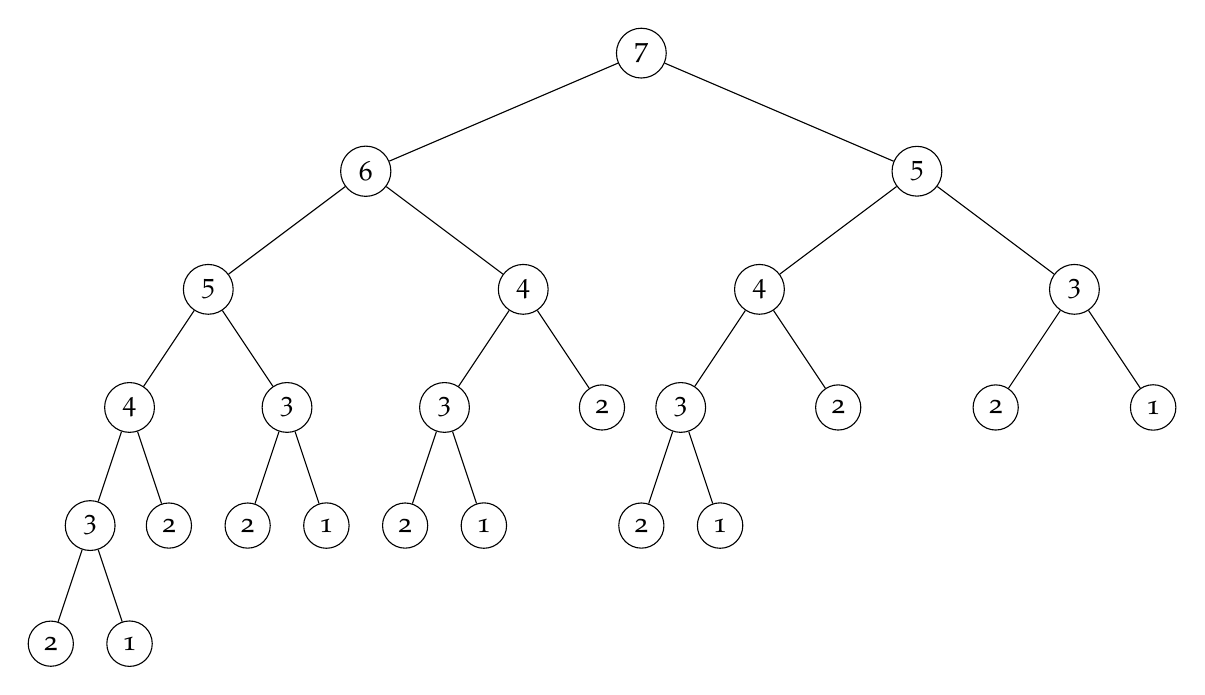
\begin{tikzpicture}[
  every node/.style = {minimum width = 1em, draw, circle},
  level/.style = {sibling distance = 80mm/#1},
  level 1/.style = {sibling distance = 70mm},
  level 2/.style = {sibling distance = 40mm},
  level 3/.style = {sibling distance = 20mm},
  level 4/.style = {sibling distance = 10mm},
  level 5/.style = {sibling distance = 10mm},
  ]
  \node {7}
  child {node {6} 
        child {node {5}
        		   child {node {4}
		   			   child {node {3}
					           child {node {2}}
		                        child {node {1}}
					           }
					   child {node {2}}
		   			  }
		       child {node {3}
		               child {node {2}}
		               child {node {1}}
		       	      }
        }
        child {node {4}
               child {node {3}
                       child {node {2}}
		               child {node {1}}
                       }
               child {node {2}}
              }
        }
  child {node {5}
         child {node {4}
                child {node {3}
                        child {node {2}}
		                child {node {1}}
                        }
                child {node {2}}
               }
         child {node {3}
         		child {node {2}}
			    child {node {1}}
                }
        };
\end{tikzpicture}
\end{document}

